\subsection{Správa paměti}
Správa paměti je v soubor metod, které operační systém používá při \textbf{přidělování operační paměti jednotlivým spuštěným procesům}.

\subsubsection*{Výhody Automatické správy paměti}
\begin{itemize}
\item Programátor se může věnovat řešení skutečného problému.
\item Rozhraní modulů jsou přehlednější -- není třeba řešit problém zodpovědnosti za uvolnění paměti pro objekty vytvořené různými moduly.
\item Nastává \textbf{menší množství chyb} spojených s přístupem do paměti.
\item Správa paměti je často pro nezkušené uživatele mnohem \textbf{efektivnější}.
\end{itemize}

\subsubsection*{Nevýhody Automatické správy paměti}
\begin{itemize}
\item Paměť může být zachována jen proto, že je dostupná, i když není dále využita.
\item Automatická správa paměti není k dispozici ve starších, ale často používaných jazycích.
\item Může navíc využívat další zdroje PC a mít tak dopad na výkon (GC).
\end{itemize}

\subsection{Úrovně správy paměti}
\begin{itemize}
	\item \textbf{Technické vybavení} -- registry, cache
	\item \textbf{Operační systém} -- virtuální paměť, segmentace, stránkování
	\item \textbf{Aplikace} -- přidělování paměti, regenerace paměti:
	\begin{itemize}
		\item \textbf{Manuální} -- delete, dispose, free()
		\item \textbf{Automatická} -- garbage collector
	\end{itemize}
\end{itemize}

\subsection{Správa paměti v jednotlivých jazycích}
Pro zjištění toho, které úseky paměti se již nepoužívají, je k dispozici mnoho algoritmů. Většinou spoléhá automatická regenerace paměti na informace o tom, na které bloky paměti \textbf{neukazuje žádná programová proměnná}. V zásadě existují \textbf{dvě} \textbf{skupiny} metod:
\begin{itemize}
	\item metody založené na \textbf{sledování odkazů},
	\item metody založené na \textbf{čítačích odkazů}.
\end{itemize}

\subsubsection{C}
Jazyk C umožňuje spravovat paměť staticky (automaticky) a dynamicky. \textbf{Staticky} alokované proměnné jsou umístěny do hlavní paměti (velice často s výkoným kódem programu). \textbf{Automaticky} alokované proměnné se alokují na zásobníků a vznikají/zanikají podle potřeb programu. Pro tyto proměnné platí, že jejich velikost musí být známá v čase kompilace.

\textbf{Dynamická} správa paměti je plně v \textbf{rukou programátora} a využívá se \textbf{4 funkcí} (\texttt{malloc}, \texttt{realloc}, \texttt{calloc}, \texttt{free}). Typicky je paměť alokována na haldě a přistupuje se k ní pomocí ukazatelů. 

\subsubsection{C++}
C++ poskytuje mnoho způsobů jak na správu paměti, od \textbf{automatické} po \textbf{manuální} pomocí operátorů \texttt{new} a \texttt{delete}. \textbf{Automatická správa paměti} alokovaných objektů je z velké části postavena na návrhovém vzoru \textbf{RAII} (Resource Aquisition Is Initialization) -- správa zdrojů daného objektu je vázána na jeho životnost a jeho destruktor je povinen jejich uvolnění. Jednoduše stačí získat zdroj (paměť, soubor, grafický handle, cokoli) a uložit ho do proměnné, která ho bude vlastnit a při jejím zániku (voláním destruktoru) ho také uvolní. A tím se o to můžete přestat starat, protože zbytek zařídí C++ kompilátor, který bude uvolňovat zdroje automaticky v rámci rušení lokálních proměnných na konci oboru platnosti (scope). Mezi \textbf{výhody} RAII patří:
\begin{itemize}
\item RAII uklízí nejenom paměť, ale všechny zdroje (soubory, mutex, databáze, transakce, síťové sockety).
\item Úklid je proveden okamžitě bez prodlení, přesně v čase kdy zdroj přestává být potřeba.
\item Proměnné a zdroje likviduje po skončení platnosti stejný thread, který je vytvořil.
\item Není třeba zastavovat program kvůli GC jako v případě Javy, LISPu, atd.
\end{itemize}
Má však i \textbf{nevýhody}:
\begin{itemize}
\item Je nepatrně pomalejší, protože dealokuje okamžitě jeden podruhém, zatímco klasické GC dealokují naráz větší množství paměti.
\item Je třeba podpoře RAII věnovat pozornost při implementaci tříd (implementace destruktoru).
\end{itemize}

\textbf{Smart pointry} představují další způsob jak na automatickou správu paměti dynamicky alokovaných objektů. SP jsou definované jako třída, která overloaduje operátory \texttt{->}, \texttt{*}, \texttt{->*}, což ji umožňuje ,,chovat se jako pointer'' a fungovat ve většině kódu v kombinaci s reálnými a smart pointry. Existuje mnoho typů, které definují typ vlastnictví a podmínky, za nichž je objekt dealokován (\texttt{shared\_ptr}, \texttt{weak\_ptr}, \texttt{unique\_ptr}). Princip dealokace je stejný jako u RAII.

\subsubsection{C\#}
Správa paměti je v jazyce C\# \textbf{plně automatizovaná}, paměťový prostor se přiděluje operátorem \textbf{new} a jeho uvolnění zajistí systém \textbf{řízení běhu programu}. V \textbf{.NET} se používá varianta GC v podobě \textbf{Mark \& Sweep}.

V případě, že pracujeme s \textbf{neřízenými zdroji} (systémové zdroje -- soubory, připojení k DB, síť), které je třeba \textbf{explicitně uvolnit}, implementuje se rozhraní \textbf{IDisposable}. To předepisuje jedinou metodu \texttt{Dispose()}, kterou je třeba zavolat po skončení práce s objektem (stará se o uvolnění zdrojů, samotný objekt poté existuje dál až do uvolnění GC).

Dále lze v .NET definovat u tříd i tzv. safe-guard v podobě \textbf{finalizer} (metoda, která se volá při uklízení objektu pomocí GC). Syntaxe je podobná C++ (\texttt{\textasciitilde{}ClassName()}). Jelikož však zhoršuje efektivitu, definuje se pouze u tříd s rozhraním IDisposable. Jeho cílem je uvolnit zdroje, \textbf{pokud uživatel objektu nezavolá/zapomene zavolat} metodu \texttt{Dispose()}. 

\subsubsection{Java}
V jazyce Java je správa paměti rovněž \textbf{plně automatizovaná} a o její uvolnění se stará GC (varianta Mark \& Sweep). Java uchovává všechny reference na Stacku a na heapu vytváří objekty. Programátor má možnost vytvářet \textbf{strong} (klasická), \textbf{weak} (pokud na objekt ukazují pouze weak reference, tak bude uvolněn), \textbf{soft} (zajištěno uvolnění při nedostatku paměti před vyhozením chyby \texttt{outOfMemory}) reference, které definují kdy bude objekt dealokován.

Speciálním případem jsou Stringy (jsou \textbf{immutable}), kdy Java spravuje tzv. \textbf{String pool}. To znamená, že si ukládá a snaží se stringy znovupoužívat jak je to možné. To neplatí pro stringy, které jsou vypočítány, pouze pro konstanty. Můžeme však přinutit JVM k vložení těchto stringů do poolu pomocí metody \texttt{.intern()}. V Javě existují \textbf{3 typy GC}:
\begin{itemize}
\item \textbf{Serial GC} -- kolektor, který běží pouze v jednom jádře (malé aplikace, malé využití dat).
\item \textbf{Parallel GC} -- oproti serial využívá více threadů.
\item \textbf{Mostly concurent GC} -- při běhu GC vždy dojde k pozastavení aplikace, tento GC se tomu snaží předejít tak, že jede \textbf{souběžně} s aplikací. Nefunguje však souběžně 100\% času, kdy je někdy nutné program pozastavit, tyto pauzy se však snaží být co nejkratší pro zajištění co nejlepšího výkonu.
\end{itemize}

Podobně jako v C\#, Java poskytuje rozhraní \texttt{AutoCloseable}, které poskytuje operaci \texttt{close()}. Nejedná se o přímého zástupce za IDisposable, ale toto rozhranní umožňuje v javě využívat tzv. \textbf{try-with-resources} (ekvivalent v C\# using), kdy dochází k automatickému zavolání metody \texttt{close()} na konci \texttt{try-catch} bloku v části \texttt{finally}.

\subsection{Garbage collector (GC)}
Je obvykle část běhového prostředí (programovacího) jazyka, nebo přídavná knihovna (podporovaná kompilátorem, hardware, operačním systémem, nebo jakoukoli kombinací těchto tří). Má za úkol \textbf{automaticky} \textbf{určit}, která část \textbf{paměti} programu je už \textbf{nepoužívaná}, a připravit ji pro další znovupoužití.

\subsubsection{Mark \& Sweep}
Algoritmus nejdříve nastaví všem objektům, které jsou v paměti, \textbf{speciální příznak} navštíven na hodnotu ne. Poté projde všechny objekty, ke kterým se lze dostat. Těm, které takto navštívil, nastaví příznak na hodnotu ano. V okamžiku, kdy se už nemůže dostat k žádnému dalšímu objektu, znamená to, že všechny objekty s příznakem navštíven majícím hodnotu ne jsou odpad -- a mohou být tedy uvolněny z paměti.

Tato metoda má několik nevýhod. Největší je, že při garbage collectionu je \textbf{přerušen běh programu}. To znamená,že programy \textbf{pravidelně zamrznou}, takže je nemožné pracovat s aplikacemi pracujícími v reálném čase.

\subsubsection{Reference counting}
Ke každému objektu je přiřazen \textbf{čítač referencí}. Když je objekt vytvořen, jeho čítači je nastaven na \textbf{hodnotu 1}. V okamžiku, kdy si nějaký jiný objekt uloží referenci na tento objekt, hodnota čítače je \textbf{zvětšena o 1}. Ve chvíli, kdy je reference mimo rozsah platnosti (např. po opuštění funkce, která si referenci uložila), nebo když je referenci přiřazena nová hodnota, čítač je \textbf{snížen o 1}. Jestliže je hodnota čítače některého objektu nulová, může být tento objekt uvolněn z paměti.

\subsubsection{Generační algoritmus}
Staví na \textbf{dvou základních principech}:
\begin{itemize}
\item Mnoho objektů se stane \textbf{odpadem} krátce \textbf{po} svém \textbf{vzniku}.
\item Jen malé procento \textbf{referencí} ve „starších“ objektech \textbf{ukazuje na objekty mladší}.
\end{itemize}
\textbf{Rozděluje si paměť programu do několika částí}, tzv. „\textbf{generací}“. Objekty jsou vytvářeny ve spodní (nejmladší) generaci a po splnění určité podmínky, obvykle stáří), jsou přeřazeny do starší generace. Pro každou generaci může být \textbf{úklid} prováděn v rozdílných \textbf{časových intervalech }(nejkratší intervaly obvykle budou platit pro nejmladší generaci) a dokonce pro rozdílné generace mohou být použity \textbf{rozdílné algoritmy úklidu}. V okamžiku, kdy se prostor pro spodní generaci zaplní, všechny dosažitelné objekty v nejmladší generaci jsou zkopírovány do starší generace. I tak bude množství kopírovaných objektů pouze zlomkem z celkového množství mladších objektů, jelikož většina z nich se již stala odpadem.

\subsubsection{Nevýhody GC}
\begin{itemize}
\item Garbage collector potřebuje ke své práci \textbf{procesorový čas}, aby mohl rozhodovat o tom, jestli je objekt v paměti „mrtvý“, nebo „živý“.
\item Některé garbage collectory mohou způsobit i dosti znatelné \textbf{pauzy}, což je vážný problém pro systémy běžící v reálném čase.
\item O stavu objektů musí mít garbage collector uloženou informaci. Tyto informace vyžadují určitou \textbf{paměť navíc}.
\item Některé jazyky s garbage collectorem neumožňují programátorovi \textbf{znovupoužití paměti}, i když ví, že paměť už nebude použita. To vede k \textbf{nárůstu alokace paměti}.
\end{itemize}

\subsection{Virtuální stroj}
Je v informatice software, který vytváří \textbf{virtualizované prostředí} mezi platformou počítače (HW i SW) a operačním systémem, ve kterém koncový uživatel může provozovat software na \textbf{abstraktním stroji}.

\subsubsection{Hardwarový virtuální stroj}
Původní význam pro virtuální stroj, někdy nazývaný též hardwarový virtuální stroj, označuje \textbf{několik jednotlivých totožných pracovních prostředí na jediném počítači}, z nichž na každém běží operační systém. Díky tomu může být aplikace psaná pro jeden OS používána na stroji, na kterém běží jiný OS, nebo zajišťuje vykonání sandboxu, který poskytuje větší úroveň izolace mezi procesy, než je dosaženo při vykonávání několika procesů najednou (multitasking) na stejném OS.

Jedním využitím může být také poskytnutí iluze mnoha uživatelům, že používají celý počítač, který je jejich „soukromým“ strojem, izolovaným od ostatních uživatelů, přestože všichni používají jeden fyzický stroj. Další výhodou může být to, že start (bootování) a restart virtuálního počítače může být mnohem rychlejší, než u fyzického stroje, protože mohou být přeskočeny úkoly jako například inicializace hardwaru.

Podobný software je často označován termíny jako virtualizace a virtuální servery. Hostitelský software, který poskytuje tuto schopnost je často označovaný jako \textbf{hypervisor} nebovirtuální strojový monitor (virtual machine monitor).
\textbf{Softwarové virtualizace} mohou být prováděny \textbf{ve třech hlavních úrovních}:
\begin{itemize}
\item \textbf{Emulace} -- virtuální stroj simuluje kompletní hardware, dovolující provoz nemodifikovaného OS na úplně jiném procesoru.
\item\textbf{Paravirtualizace} -- virtuální stroj nesimuluje hardware, ale místo toho nabídne \textbf{speciální rozhraní API}, které vyžaduje určité modifikace hostovaného operačního systému, aby mohl být tento OS nad virtuálním strojem spouštěn.
\item\textbf{Nativní virtualizace} a „\textbf{plná virtualizace}“ -- virtuální stroj jen částečně simuluje dost hardwaru, aby mohl nemodifikovaný OS běžet samostatně, ale hostitelský OS musí být určený pro stejný druh procesoru. Pojem nativní virtualizace se někdy používá ke zdůraznění, že je \textbf{využita hardwarová podpora pro virtualizaci} (tzv. virtualizační technologie) (WMware, Parallels).
\end{itemize}

\subsubsection{Aplikační virtuální stroj}
Dalším významem termínu virtuální stroj je počítačový software, který\textbf{ izoluje aplikace používané uživatelem na počítači}. Protože verze virtuálního stroje jsou psány pro \textbf{různé počítačové platformy}, jakákoliv aplikace psaná pro virtuální stroj může být provozována na kterékoli z platforem, místo toho, aby se musely vytvářet oddělené verze aplikace pro každý počítač a operační systém. Aplikace běžící na počítači používá \textbf{interpret} nebo \textbf{Just in time kompilaci}. 

Jeden z nejlepších známých příkladů aplikačního virtuálního stroje je \textbf{Java Virtual Machine} (\textbf{JVM}) od firmy Sun Microsystem. Java Virtual Machine umí zpracovat mezikód (\textbf{Java bytecode}), který je obvykle vytvořen ze zdrojových kódů programovacího jazyka Java. Díky tomu, že je JVM k dispozici na mnoha platformách, je možné aplikaci v Javě vytvořit pouze jednou a spustit na kterékoliv z platforem, pro kterou je vyvinut JVM (např. Windows, Linux).

\subsubsection{Virtuální prostředí}
Virtuální prostředí (jinak virtuální soukromý server) je jiný druh virtuálního stroje. Ve skutečnosti, to je \textbf{virtualizované prostředí} pro běh programů \textbf{na úrovni uživatele} (tj. ne jádra operačního systému a ovladače, ale aplikace). Virtuální prostředí jsou vytvořena použitím softwaru zavádějícího virtualizaci na úrovni operačního systému, jako například Virtuozzo, OpenVZ. Příkladem může být \textbf{VPS} u poskytovatelů stránek.

\subsection{Podpora paralelního zpracování}
\textbf{Paralelně programovaný software} využívá možnost rozdělení jednoho velkého výpočetního problému na několik menších problémů, které jsou řešeny „\textbf{současně}". Prvky sloužící k paralelnímu zpracování výpočtu mohou být různé. Jedná se například o jeden \textbf{počítač s více procesory}, \textbf{několik počítačů }v síti, \textbf{specializovaný hardware} nebo \textbf{kombinaci} těchto prvků.

\subsection{Thread}
Operační systémy používají pro oddělení různých běžících aplikací procesy. \textbf{Proces} je tvořen paměťovým prostorem a jedním nebo více vlákny. \textbf{Vlákno je samostatně prováděný výpočetní tok} (posloupnost instrukcí), který běží v rámci procesu. Každému vláknu přísluší vlastní priorita a řada systémových struktur.

Operační systémy s \textbf{preemptivním} \textbf{multitaskingem} vytvářejí dojem souběžného provádění více vláken ve více procesech. To je zajištěno rozdělením času procesoru mezi jednotlivá vlákna po malých časových intervalech. Pokud časový interval vyprší, je běžící vlákno pozastaveno, uloží se jeho kontext a obnoví se kontext dalšího vlákna ve frontě, jemuž je pak předáno řízení. Vzhledem k tomu, že tyto časové úseky jsou z pohledu uživatele velmi krátké, je výsledný dojem i na počítači s jediným procesorem takový, jako by pracovalo více vláken současně. V případě, že máme k dispozici více procesorů, jsou mezi ně vlákna přidělována ke zpracování a k současnému běhu pak skutečně dochází.

Přepnutí mezi vlákny bývá výrazně rychlejší než v procesovém multitaskingu, neboť vlákna \textbf{sdílejí stejnou paměť }a uživatelská práva svého mateřského procesu a není je třeba při přepínání měnit. Vlákno také spotřebuje méně paměti a je rychlejší na vytváření.

Vlákna je možné vytvořit i čistě na \textbf{aplikační úrovni} bez nativní podpory operačního systému (využitím sdílené paměti a dalších technik). Takto vzniklá vlákna je poté možné spouštět postupně v jednotlivých procesech operačního systému nebo takzvaně m:n, tedy v několika vláknech operačního systému současně spouštět větší počet aplikačních vláken. 

Samotným zvyšováním počtu vláken však obvykle odpovídajícího zvýšení výkonu aplikace nedosáhneme. Naopak se doporučuje, abychom používali co nejméně vláken a tím omezili spotřebu systémových prostředků a nárůst režie. Typické problémy jsou následující:

\begin{itemize}
\item Pro ukládání kontextových informací se \textbf{spotřebovává dodatečná paměť}, a tedy celkový počet procesů a vláken, které mohou v systému současně existovat, je \textbf{omezený}.
\item Obsluha velkého počtu vláken \textbf{spotřebovává významnou část času procesoru}. Existuje-li tedy příliš mnoho vláken, většina z nich příliš významně nepostupuje. Navíc pokud je většina vláken v jednom procesu, dostávají se vlákna jiných procesů na řadu méně často.
\item Organizace programu s mnoha vlákny je složitá a může být zdrojem mnoha chyb. Zejména je obtížné zajistit jejich \textbf{správnou synchronizaci}.
\end{itemize}

\subsubsection{Shrnutí}
\begin{itemize}
	\item Vlákno je \textbf{odlehčený proces}, pomocí něhož se snižuje režie OS při změně kontextu (umožňuje multitasking).
	\item Vlákno je \textbf{samostatně prováděný výpočetní tok}.
	\item Vlákna běží v \textbf{rámci procesu}.
	\item Vlákna jednoho procesu běží v rámci stejného prostoru paměti. \textbf{Sdílí jeho prostředky a paměť}.
	\item Každé vlákno má vyhrazený prostor pro specifické proměnné (runtime prostředí).
	\item Pokud běží v jádře OS dochází k \textbf{paralelizaci}, simulování threadů v aplikaci paralelizaci pouze simuluje.
\end{itemize}

\subsection{Kdy použít vlákna?}
Vlákna je výhodné použít, pokud aplikace splňuje některé následující kritérium:
\begin{itemize}
	\item Je \textbf{složena}\textbf{ z nezávislých úloh}.
	\item Může být \textbf{blokována} po dlouho dobu.
	\item Obsahuje \textbf{výpočetně náročnou} část.
	\item Musí reagovat na asynchronní události.
	\item Obsahuje úlohy s nižší nebo vyšší prioritou než zbytek aplikace.
\end{itemize}

\subsubsection{Typické aplikace}
\begin{itemize}
	\item \textbf{Servery} -- obsluhují více klientů najednou. Obsluha typicky znamená \textbf{přístup k několika sdíleným zdrojům} a hodně vstupně výstupních operací (I/O).
	\item \textbf{Výpočetní aplikace} -- na \textbf{víceprocesorovém systému} lze výpočet urychlit rozdělením úlohy na více procesorů.
	\item \textbf{Aplikace reálného času} -- lze využít specifických rozvrhovačů. Více vláknová aplikace je výkonnější než složité asynchronní programování, neboť vlákno čeká na příslušnou událost namísto přerušování vykonávání kódu a přepínání kontextu.
\end{itemize}

\subsection{Vlákna v Javě}
Každé vlákno v Javě je instancí třídy \texttt{java.lang.Thread}. Tato třída zajišťuje spuštění, zastavení a ukončení vlákna. Vlákno musí implementovat metodu \textbf{run}, která definuje činnost vlákna. Této metodě je předáno řízení po spuštění vlákna metodou \texttt{start}.

\subsubsection{Životní cyklus}
Vlákno v průběhu svého života prochází posloupností následujících stavů:
\begin{itemize}
\item \textbf{New} -- bezprostředně po vytvoření ještě nejsou vláknu přiděleny žádné systémové prostředky, vlákno neběží.
\item \textbf{Runnable} -- v tomto stavu se nachází po provedení metody \texttt{start()}, scheduler jej však nezvolil, aby byl běžící.
\item \textbf{Running} -- vlákno běží, do tohoto stavu se dostane po té co jej vybere scheduler.
\item \textbf{Not runnable (Blocked)} -- vlákno je pozastaveno voláním jedné s metod \texttt{sleep}, \texttt{wait} nebo \texttt{suspend}, případně čeká na dokončení operace vstupu/výstupu.
\item \textbf{Terminated} -- thread je ukončen nebo ve stavu \textbf{Dead} pokud existuje metoda run.
\end{itemize}

\subsection{Hlavní problémy vícevláknových aplikací}
\begin{itemize}
\item \textbf{Deadlock (uváznutí)} -- je situace, kdy úspěšné dokončení první akce je \textbf{podmíněno předchozím dokončením druhé akce}, přičemž druhá akce může být dokončena až po dokončení první akce. Deadlocku můžeme zabránit například tím, že proces musí o \textbf{všechny prostředky}, které potřebuje, zažádat \textbf{najednou}. Buď je všechny dostane, nebo nedostane ani jeden. 
\item \textbf{Souběh (race conditions)} -- \textbf{přístup více vláken ke sdíleným proměnným} a alespoň jedno vlákno nevyužívá synchronizačních mechanismů. Vlákno čte hodnotu, zatímco jiné vlákno zapisuje. Zápis a čtení nejsou atomické a data mohou být neplatná. K zabránění souběhu se používají \textbf{zámky} (lock), jejichž použitím se zajistí, že jen jedno vlákno může v jeden okamžik přistoupit k označenému resource souboru nebo části kódu.
\item \textbf{Starvation (vyhladovění)} -- stav, kdy jsou vláknu neustále odepírány prostředky. Bez těchto prostředků program nikdy nedokončí svůj úkol.
\end{itemize}

\begin{figure}[H]
\centering
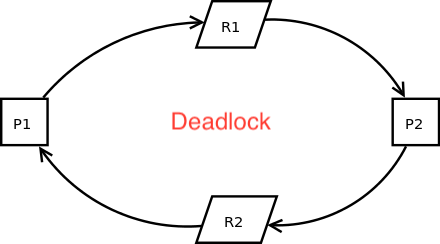
\includegraphics[width=.4\textwidth]{assets/deadlock.png}
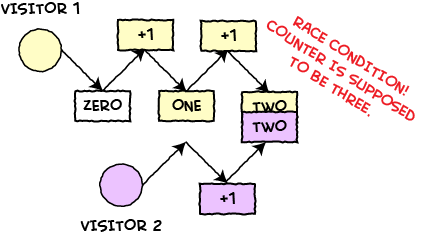
\includegraphics[width=.4\textwidth]{assets/race_condition.png}
\end{figure}

\subsection{Mechanismy synchronizace}
\begin{itemize}
	\item \textbf{Mutex} -- zámek kritické sekce.
	\item \textbf{Podmíněná proměnná} (condition variable) synchronizace hodnotou proměnné. Čekání vlákna na probuzení od jiného vlákna.
	\item \textbf{Semafor} --  čítač, definuje kolik procesů může max přistupovat k nějakému zdroji.
\end{itemize}

\subsubsection{Mutex}
Mutex = mutual exclusion, neboli vzájemné vyloučení je algoritmus používaný v programování jako \textbf{synchronizační prostředek}. Zabraňuje tomu, aby byly současně vykonávány dva (nebo více) kódy nad stejným sdíleným prostředkem. Základní operace:
\begin{itemize}
	\item \textbf{Lock} -- uzamknutí mutexu (přiřazení mutexu vláknu). Pokud nelze mutex získat, vlákno přechází do blokovaného režimu a čeká na uvolnění zámku.
	\item \textbf{Unlock} -- uvolnění zámku. Pokud jiná vlákna čekají na uvolnění, je vybráno jedno vlákno, které mutex získá.
	\item \textbf{Rozšířené metody:}
	\begin{itemize}
		\item \textbf{Rekursivní} -- vícenásobné zamykání stejným vláknem.
		\item \textbf{Try} -- okamžitý návrat pokud není možné mutex získat.
		\item \textbf{Timed} -- pokus o získání zámku s omezenou dobou čekání.
	\end{itemize}
\end{itemize}

\subsubsection{Semafor}
Semafory jsou velmi podobné mutexům. Zatímco mutex má jen dva stavy – zamknut/odemknut, semafor jich může mít víc. Semafor je v podstatě \textbf{čítač}, který může být \textbf{zmenšován} a \textbf{zvětšován}. Když je čítač roven \textbf{nule} je semafor považován za \textbf{zamčený}, v opačném případě je \textbf{odemčen}. Semafory se používají, pokud máme omezený počet nějakých zdrojů. Pokud nějaké vlákno chce ke zdroji přistupovat, zmenší hodnotu semaforu. Pokud semafor nebyl roven nule, proces pokračuje dál, v opačném případě čeká, až jiné vlákno přestane zdroj používat a hodnotu semaforu zvětší.

\subsection{Rozdělování práce vláknům}
Modely řeší způsob \textbf{vytváření} a \textbf{rozdělování práce} mezi vlákna:
\begin{itemize}
	\item \textbf{Boss/Worker} -- hlavní vlákno, řídí rozdělení úlohy jiným vláknům.
	\item \textbf{Peer} -- vlákna běží paralelně bez specifického vedoucího.
	\item \textbf{Pipeline} -- zpracování dat sekvencí operací. Předpokládá dlouhý vstupní proud dat.
\end{itemize}